\subsection{Integrales dobles en recintos generales}

Cuando hablamos de recintos generales,
nos referimos a recintos no rectangulares.

Se distinguen dos casos: 
\begin{itemize}
    \item En \(x\) es un intervalo y en \(y\) funciones \(f(x)\)
    \item En \(x\) tenemos funciones \(f(y)\) y en \(y\) un intervalo
\end{itemize}

Para operar estas integrales es necesario:

\begin{enumerate}
    \item Graficar el recinto
    \item Determinar intersecciones 
    \item Plantear integral y operar
\end{enumerate}

\subsection{Ejemplo}

Calcular volumen para superficie \(z = x + 2y\),
en el recinto delimitado por \(y = x^{2}\) e \(y = x + 2\).

Primero,
graficamos recinto:

\begin{table}
    \centering
    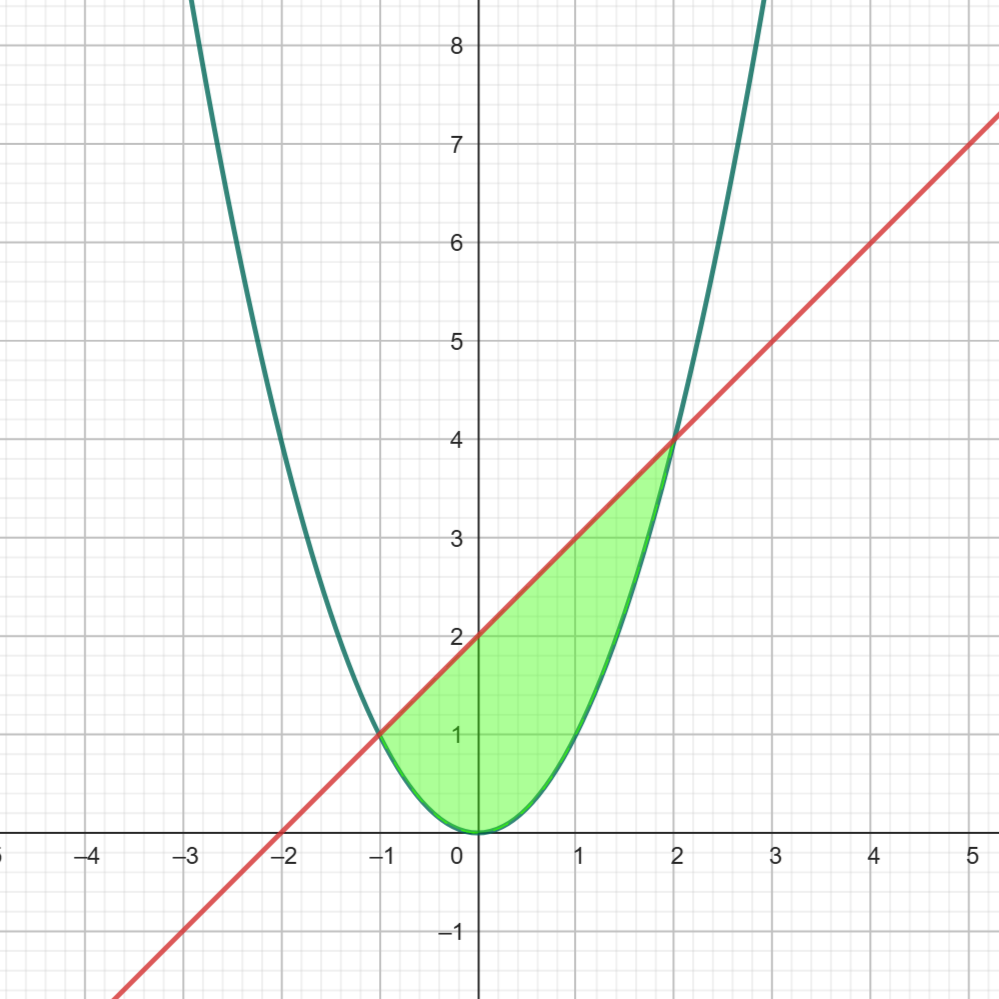
\includegraphics[width=\textwidth]{./img/01.png}
    \caption{Recinto}
\end{table}

Determinamos intersecciones en \(x\):

\begin{align*}
    x^{2} = x + 2 \\
    x^{2} - x = 2 \\
    (x-\frac{1}{2})^{2} = \frac{9}{4} \\
    |x-\frac{1}{2}| = \frac{3}{2} \\
    x = \frac{1}{2} \pm \frac{3}{2} \\ 
    x = 2 \land x = x = -1 \\
\end{align*}

Planteamos integral:

\begin{align*}
    \int_{-1}^{2} [\int_{x^{2}}^{x+2} x + 2y \,dy] \,dx
\end{align*}

Resolvemos primera integral:

\begin{align*}
    \int_{x^{2}}^{x+2} x + 2y \,dy & = \int_{x^{2}}^{x+2} x \,dy + \int_{x^{2}}^{x+2} 2y \,dy \\
    & = xy|_{x^{2}}^{x+2} + y^{2}|_{x^{2}}^{x+2} \\
    & = x^{2} + 2x - x^{3} + (x+2)^{2} - x^{4} \\
    & = x^{2} + 2x - x^{3} + x^{2} + 2x + 4 - x^{4} \\
    & = -x^{4} - x^{3} + 2x^{2} + 4x + 4 \\
\end{align*}

Operamos segunda integral.
Como vemos, si operamos primero la dependiente,
queda un polinomio en función de la otra para el final: 

\begin{gather*}
    \int_{-1}^{2} -x^{4} - x^{3} + 2x^{2} + 4x + 4 \,dx = \left.-\frac{x^{5}}{5} - \frac{x^{4}}{4} + \frac{2x^{3}}{3} + 2x^{2} + 4x\right|_{-1}^{2} \\
    -\frac{2^{5}}{5} - \frac{2^{4}}{4} + \frac{2\cdot2^{3}}{3} + 2\cdot2^{2} + 8 + \frac{(-1)^{5}}{5} + \frac{(-1)^{4}}{4} - \frac{2(-1)^{3}}{3} - 2(-1)^{2} + 4 \\
    -\frac{32}{5} - 4 + \frac{16}{3} + 8 + 8 - \frac{1}{5} + \frac{1}{4} + \frac{2}{3} - 2 + 4 \\
    \frac{67}{5} + \frac{1}{4} \\
    \boxed{\frac{263}{20}} \\
\end{gather*}